\documentclass[border=3pt]{standalone}
% Preâmbulo compartilhado pelos diagramas TikZ da aula 6 de IHR (Interação Verbal)
\usepackage[T1]{fontenc}
\usepackage[utf8]{inputenc}
\usepackage{lmodern}
\usepackage{amsmath}
\usepackage{xcolor}
\usepackage{tikz}
\usetikzlibrary{arrows.meta,angles,quotes,decorations.pathmorphing,decorations.pathreplacing,calc,
                positioning,shapes.geometric,shapes.misc,backgrounds,fit,
                math}

% Paleta (mesma dos SVGs originais)
% Paleta da disciplina de IHR: acento azul (#1A6FB5), cor de destaque do tema.
% (o nome "dblue" é mantido para não alterar todos os diagramas)
\definecolor{dblue}{HTML}{1A6FB5}
\definecolor{dorange}{HTML}{B3541E}
\definecolor{dgreen}{HTML}{4A7C59}
\definecolor{dred}{HTML}{9C4B4B}
\definecolor{dcream}{HTML}{F4F1EA}
\definecolor{dshade}{HTML}{DDD7C9}

% Função gaussiana (não normalizada por padrão de escala visual)
\pgfmathdeclarefunction{gauss}{3}{%
  \pgfmathparse{1/(#3*sqrt(2*pi))*exp(-((#1-#2)^2)/(2*#3^2))}%
}

% Estilos comuns (prefixo d... para não colidir com chaves internas do pgf)
\tikzset{
  >={Stealth[length=2mm]},
  dguide/.style={gray!55, dashed, line width=0.4pt},
  daxis/.style={gray!60, line width=0.7pt, ->},
  dbody/.style={fill=black!3, draw=black!80, line width=1pt},
  dacc/.style={draw=dblue, line width=1pt},
  dlbl/.style={black!55, font=\small},
  dsub/.style={black!45, font=\footnotesize},
  dstate/.style={circle, draw=black!80, fill=dcream, line width=1pt,
                 minimum size=17mm, font=\large, inner sep=1pt},
  dobs/.style={circle, draw=black!80, fill=dshade, line width=1pt,
               minimum size=14mm, font=\large, inner sep=1pt},
  dbox/.style={rounded corners=2pt, draw=black!80, fill=dcream, line width=1pt,
               align=center, inner sep=6pt},
  dop/.style={circle, draw=black!80, fill=white, line width=1pt,
              minimum size=6mm, inner sep=0pt, font=\small},
  dtrans/.style={->, dblue, line width=1pt},
  dmeas/.style={->, dorange, line width=1pt},
  dcurve/.style={line width=1pt, dblue},
  dcurveb/.style={line width=1.4pt, dorange},
}

\usetikzlibrary{shapes.callouts}
\begin{document}
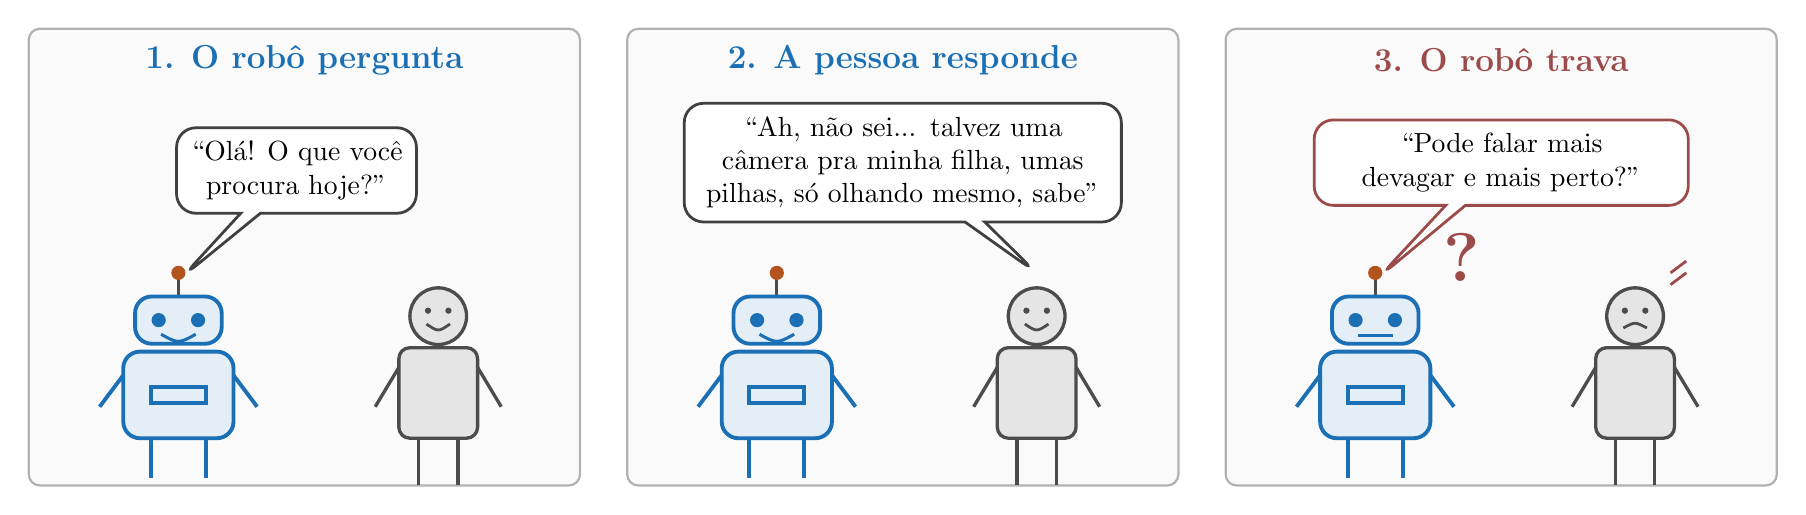
\begin{tikzpicture}[x=1cm,y=1cm,
  bal/.style={rectangle callout, rounded corners=7pt, draw=black!75, fill=white, line width=1pt, align=center, font=\normalsize, inner sep=5pt}]

  \newcommand{\robo}[3]{% x y tipo (0 normal,1 confuso)
    \begin{scope}[shift={(#1,#2)}]
      \draw[black!70, line width=1pt] (0,1.55) -- (0,1.85); \fill[dorange] (0,1.9) circle (0.09);
      \draw[dblue, fill=dblue!12, line width=1.4pt, rounded corners=6pt] (-0.55,1.0) rectangle (0.55,1.6);
      \fill[dblue] (-0.25,1.3) circle (0.09); \fill[dblue] (0.25,1.3) circle (0.09);
      \ifnum#3=1 \draw[dblue, line width=1.1pt] (-0.22,1.1) -- (0.22,1.1); \else \draw[dblue, line width=1.1pt] (-0.22,1.12) .. controls (0,1.0) .. (0.22,1.12); \fi
      \draw[dblue, fill=dblue!12, line width=1.4pt, rounded corners=6pt] (-0.7,-0.2) rectangle (0.7,0.9);
      \draw[dblue, line width=1.4pt] (-0.7,0.6) -- (-1.0,0.2); \draw[dblue, line width=1.4pt] (0.7,0.6) -- (1.0,0.2);
      \draw[dblue, line width=1.4pt] (-0.35,-0.2) -- (-0.35,-0.7); \draw[dblue, line width=1.4pt] (0.35,-0.2) -- (0.35,-0.7);
      \draw[dblue, fill=dblue!12, line width=1.4pt] (-0.35,0.45) rectangle (0.35,0.25);
    \end{scope}}
  \newcommand{\pessoa}[3]{%
    \begin{scope}[shift={(#1,#2)}]
      \draw[black!70, fill=black!10, line width=1.2pt] (0,1.35) circle (0.36);
      \fill[black!70] (-0.13,1.42) circle (0.04); \fill[black!70] (0.13,1.42) circle (0.04);
      \ifnum#3=1 \draw[black!70, line width=1pt] (-0.15,1.2) .. controls (0,1.28) .. (0.15,1.2); \else \draw[black!70, line width=1pt] (-0.15,1.25) .. controls (0,1.15) .. (0.15,1.25); \fi
      \draw[black!70, fill=black!10, line width=1.2pt, rounded corners=4pt] (-0.5,-0.2) rectangle (0.5,0.95);
      \draw[black!70, line width=1.2pt] (-0.5,0.7) -- (-0.8,0.2); \draw[black!70, line width=1.2pt] (0.5,0.7) -- (0.8,0.2);
      \draw[black!70, line width=1.2pt] (-0.25,-0.2) -- (-0.25,-0.8); \draw[black!70, line width=1.2pt] (0.25,-0.2) -- (0.25,-0.8);
    \end{scope}}

  % painel 1
  \begin{scope}
    \draw[black!30, fill=black!2, rounded corners=4pt, line width=0.8pt] (0,0) rectangle (7,5.8);
    \node[font=\bfseries\large, dblue] at (3.5,5.4) {1. O robô pergunta};
    \robo{1.9}{0.8}{0} \pessoa{5.2}{0.8}{0}
    \node[bal, callout absolute pointer={(1.95,2.65)}] at (3.4,4.0) {``Olá! O que você\\ procura hoje?''};
  \end{scope}
  % painel 2
  \begin{scope}[shift={(7.6,0)}]
    \draw[black!30, fill=black!2, rounded corners=4pt, line width=0.8pt] (0,0) rectangle (7,5.8);
    \node[font=\bfseries\large, dblue] at (3.5,5.4) {2. A pessoa responde};
    \robo{1.9}{0.8}{0} \pessoa{5.2}{0.8}{0}
    \node[bal, callout absolute pointer={(5.2,2.7)}, text width=5.2cm] at (3.5,4.1) {``Ah, não sei... talvez uma câmera pra minha filha, umas pilhas, só olhando mesmo, sabe''};
  \end{scope}
  % painel 3
  \begin{scope}[shift={(15.2,0)}]
    \draw[black!30, fill=black!2, rounded corners=4pt, line width=0.8pt] (0,0) rectangle (7,5.8);
    \node[font=\bfseries\large, dred] at (3.5,5.4) {3. O robô trava};
    \robo{1.9}{0.8}{1} \pessoa{5.2}{0.8}{1}
    \node[dred, font=\Huge\bfseries] at (3.0,2.9) {?};
    \node[bal, draw=dred, callout absolute pointer={(1.95,2.65)}, text width=4.4cm] at (3.5,4.1) {``Pode falar mais\\ devagar e mais perto?''};
    \draw[dred, line width=1pt] (5.65,2.55) -- (5.85,2.7) (5.65,2.7) -- (5.85,2.85);
  \end{scope}
\end{tikzpicture}
\end{document}
